\documentclass[14pt]{extbook}
\usepackage{multicol, enumerate, enumitem, hyperref, color, soul, setspace, parskip, fancyhdr} %General Packages
\usepackage{amssymb, amsthm, amsmath, bbm, latexsym, units, mathtools} %Math Packages
\everymath{\displaystyle} %All math in Display Style
% Packages with additional options
\usepackage[headsep=0.5cm,headheight=12pt, left=1 in,right= 1 in,top= 1 in,bottom= 1 in]{geometry}
\usepackage[usenames,dvipsnames]{xcolor}
\usepackage{dashrule}  % Package to use the command below to create lines between items
\newcommand{\litem}[1]{\item#1\hspace*{-1cm}\rule{\textwidth}{0.4pt}}
\pagestyle{fancy}
\lhead{Progress Quiz 4}
\chead{}
\rhead{Version A}
\lfoot{8448-1521}
\cfoot{}
\rfoot{Fall 2020}
\begin{document}

\begin{enumerate}
\litem{
Choose the equation of the function graphed below.
\begin{center}
    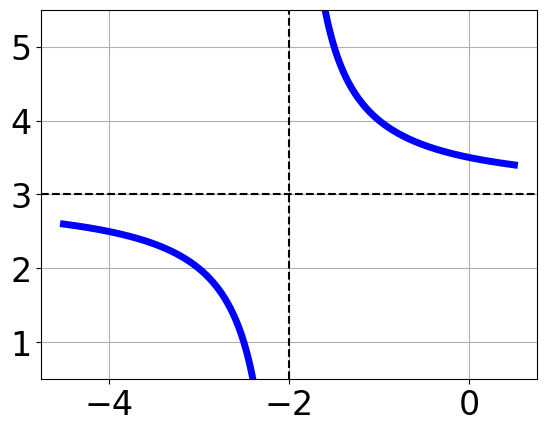
\includegraphics[width=0.5\textwidth]{../Figures/rationalGraphToEquationA.png}
\end{center}
\begin{enumerate}[label=\Alph*.]
\item \( f(x) = \frac{1}{(x - 1)^2} + 2 \)
\item \( f(x) = \frac{-1}{(x + 1)^2} + 2 \)
\item \( f(x) = \frac{-1}{x + 1} + 2 \)
\item \( f(x) = \frac{1}{x - 1} + 2 \)
\item \( \text{None of the above} \)

\end{enumerate} }
\litem{
Solve the rational equation below. Then, choose the interval(s) that the solution(s) belongs to.\[ \frac{-63}{28x + 14} + 1 = \frac{-63}{28x + 14} \]\begin{enumerate}[label=\Alph*.]
\item \( \text{All solutions lead to invalid or complex values in the equation.} \)
\item \( x \in [-0.5,0.5] \)
\item \( x \in [0.1,0.6] \)
\item \( x_1 \in [-1, -0.3] \text{ and } x_2 \in [0.2,1.1] \)
\item \( x_1 \in [-1, -0.3] \text{ and } x_2 \in [-1.2,0.2] \)

\end{enumerate} }
\litem{
Choose the graph of the equation below.\[ f(x) = \frac{-1}{x + 2} + 2 \]\begin{enumerate}[label=\Alph*.]
\begin{multicols}{2}\item 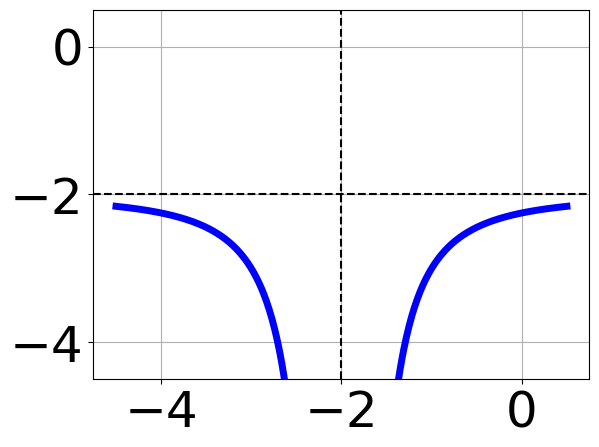
\includegraphics[width = 0.3\textwidth]{../Figures/rationalEquationToGraphAA.png}\item 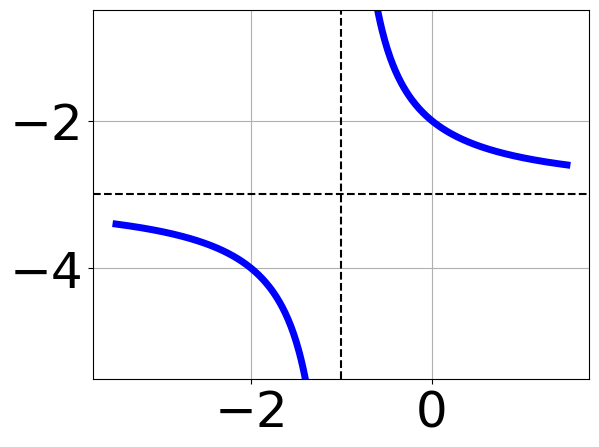
\includegraphics[width = 0.3\textwidth]{../Figures/rationalEquationToGraphBA.png}\item 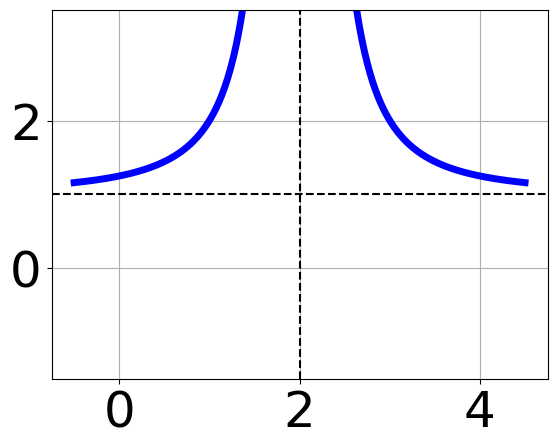
\includegraphics[width = 0.3\textwidth]{../Figures/rationalEquationToGraphCA.png}\item 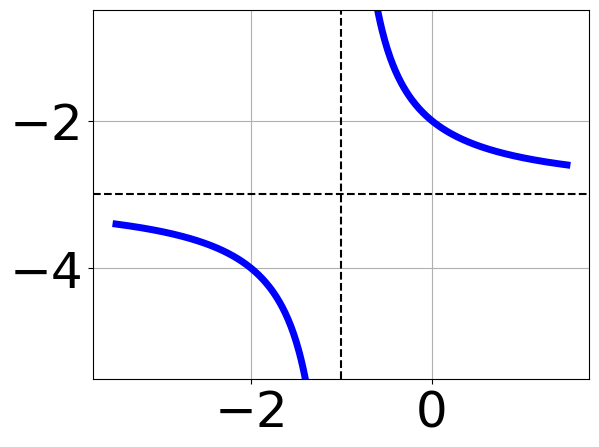
\includegraphics[width = 0.3\textwidth]{../Figures/rationalEquationToGraphDA.png}\end{multicols}\item None of the above.
\end{enumerate} }
\litem{
Solve the rational equation below. Then, choose the interval(s) that the solution(s) belongs to.\[ \frac{7x}{4x + 3} + \frac{-3x^{2}}{8x^{2} +26 x + 15} = \frac{-2}{2x + 5} \]\begin{enumerate}[label=\Alph*.]
\item \( x \in [-0.75,2.24] \)
\item \( x_1 \in [-4.13, -2.89] \text{ and } x_2 \in [-1.61,-0.48] \)
\item \( \text{All solutions lead to invalid or complex values in the equation.} \)
\item \( x \in [-3.66,-1.02] \)
\item \( x_1 \in [-4.13, -2.89] \text{ and } x_2 \in [-0.35,0.12] \)

\end{enumerate} }
\litem{
Solve the rational equation below. Then, choose the interval(s) that the solution(s) belongs to.\[ \frac{56}{56x + 32} + 1 = \frac{56}{56x + 32} \]\begin{enumerate}[label=\Alph*.]
\item \( x_1 \in [-1.57, 0.43] \text{ and } x_2 \in [-0.5,1] \)
\item \( x \in [-0.57,0.43] \)
\item \( x \in [0.57,2.57] \)
\item \( \text{All solutions lead to invalid or complex values in the equation.} \)
\item \( x_1 \in [-1.57, 0.43] \text{ and } x_2 \in [-1.5,0.4] \)

\end{enumerate} }
\litem{
Determine the domain of the function below.\[ f(x) = \frac{6}{20x^{2} +31 x + 12} \]\begin{enumerate}[label=\Alph*.]
\item \( \text{All Real numbers except } x = a, \text{ where } a \in [-0.82, -0.79] \)
\item \( \text{All Real numbers except } x = a \text{ and } x = b, \text{ where } a \in [-20.05, -19.95] \text{ and } b \in [-12.05, -11.96] \)
\item \( \text{All Real numbers.} \)
\item \( \text{All Real numbers except } x = a \text{ and } x = b, \text{ where } a \in [-0.82, -0.79] \text{ and } b \in [-0.76, -0.73] \)
\item \( \text{All Real numbers except } x = a, \text{ where } a \in [-20.05, -19.95] \)

\end{enumerate} }
\litem{
Choose the graph of the equation below.\[ f(x) = \frac{1}{x + 1} + 2 \]\begin{enumerate}[label=\Alph*.]
\begin{multicols}{2}\item 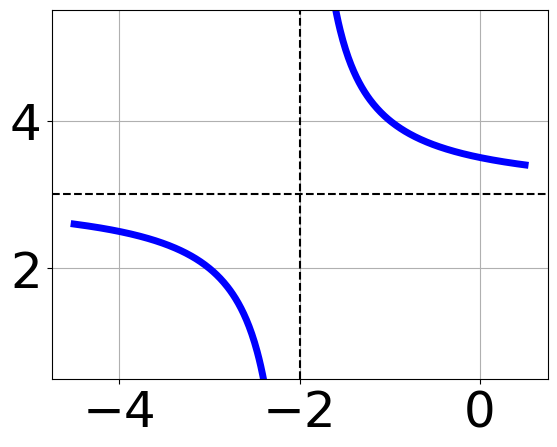
\includegraphics[width = 0.3\textwidth]{../Figures/rationalEquationToGraphCopyAA.png}\item 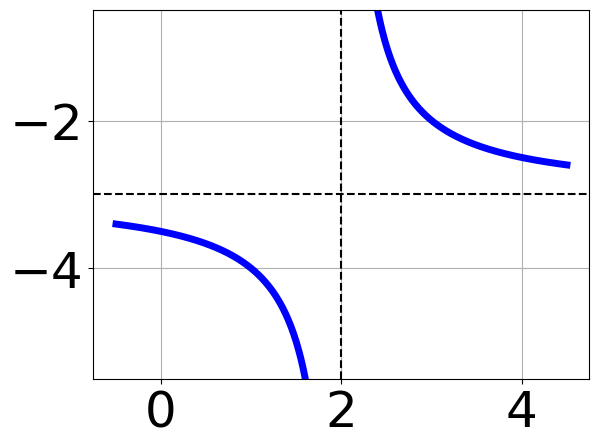
\includegraphics[width = 0.3\textwidth]{../Figures/rationalEquationToGraphCopyBA.png}\item 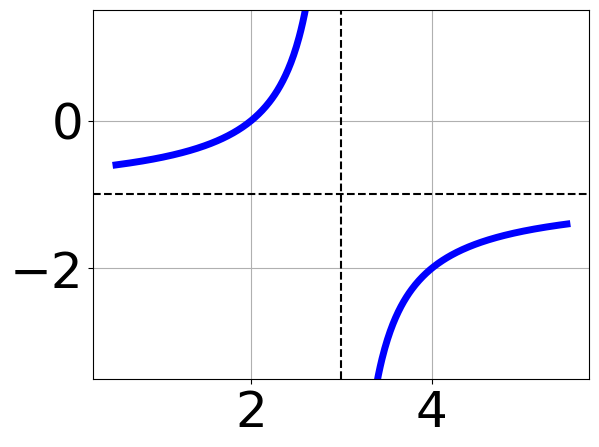
\includegraphics[width = 0.3\textwidth]{../Figures/rationalEquationToGraphCopyCA.png}\item 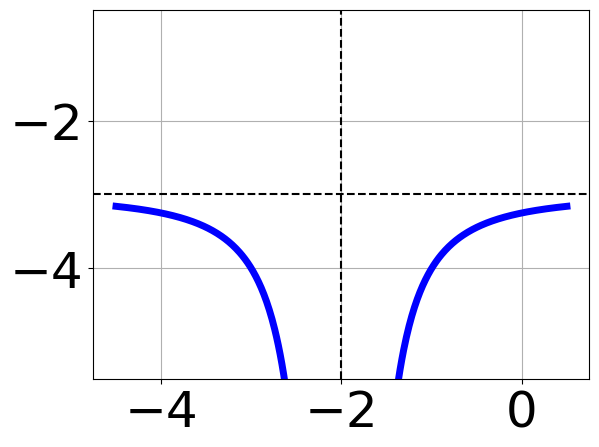
\includegraphics[width = 0.3\textwidth]{../Figures/rationalEquationToGraphCopyDA.png}\end{multicols}\item None of the above.
\end{enumerate} }
\litem{
Solve the rational equation below. Then, choose the interval(s) that the solution(s) belongs to.\[ \frac{-2x}{-4x -4} + \frac{-7x^{2}}{-8x^{2} -36 x -28} = \frac{-5}{2x + 7} \]\begin{enumerate}[label=\Alph*.]
\item \( x_1 \in [-3.29, -1.73] \text{ and } x_2 \in [-1.04,-0.9] \)
\item \( \text{All solutions lead to invalid or complex values in the equation.} \)
\item \( x_1 \in [-3.29, -1.73] \text{ and } x_2 \in [-0.91,-0.75] \)
\item \( x \in [-2.09,0.72] \)
\item \( x \in [-3.97,-3.05] \)

\end{enumerate} }
\litem{
Choose the equation of the function graphed below.
\begin{center}
    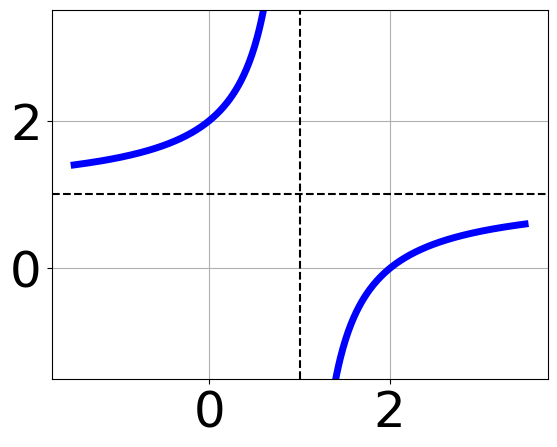
\includegraphics[width=0.5\textwidth]{../Figures/rationalGraphToEquationCopyA.png}
\end{center}
\begin{enumerate}[label=\Alph*.]
\item \( f(x) = \frac{-1}{(x + 3)^2} + 2 \)
\item \( f(x) = \frac{-1}{x + 3} + 2 \)
\item \( f(x) = \frac{1}{(x - 3)^2} + 2 \)
\item \( f(x) = \frac{1}{x - 3} + 2 \)
\item \( \text{None of the above} \)

\end{enumerate} }
\litem{
Determine the domain of the function below.\[ f(x) = \frac{4}{20x^{2} +54 x + 36} \]\begin{enumerate}[label=\Alph*.]
\item \( \text{All Real numbers except } x = a \text{ and } x = b, \text{ where } a \in [-30.02, -29.55] \text{ and } b \in [-24.02, -23.73] \)
\item \( \text{All Real numbers except } x = a, \text{ where } a \in [-1.58, -1.45] \)
\item \( \text{All Real numbers except } x = a \text{ and } x = b, \text{ where } a \in [-1.58, -1.45] \text{ and } b \in [-1.39, -1.11] \)
\item \( \text{All Real numbers except } x = a, \text{ where } a \in [-30.02, -29.55] \)
\item \( \text{All Real numbers.} \)

\end{enumerate} }
\end{enumerate}

\end{document}